
%%%%%%%%%%%%%%%%%%%%%%%%%%%%%%%%%%%%%%%%%%%%%%%%%%%%%%%%%%
%%
%% This is the "PREAMBLE". Here we define the type of document and load in any packages we might want. You can also set parameters %% % and create your own short-hand here.
%%
%%%%%%%%%%%%%%%%%%%%%%%%%%%%%%%%%%%%%%%%%%%%%%%%%%%%%%%%%%

 \documentclass[9pt]{article}
 
 \def\solutions{1}
\usepackage{mathtools}
\DeclarePairedDelimiter\ceil{\lceil}{\rceil}
\DeclarePairedDelimiter\floor{\lfloor}{\rfloor}

\usepackage{hyperref} 
 \usepackage{amsmath}
 \usepackage{amssymb}
 \usepackage{graphicx}    % needed for including graphics e.g. EPS, PS \usepackage{tikz}
 \usepackage{tikz}
 \usepackage{tikzsymbols}
 \usepackage{relsize}
 \usetikzlibrary{patterns,decorations.pathreplacing,shapes,arrows}
 \usepackage{algorithm2e}
 \topmargin -2.5cm        % read Lamport p.163
 \oddsidemargin -0.04cm   % read Lamport p.163
 \evensidemargin -0.04cm  % same as oddsidemargin but for left-hand pages
 \textwidth 16.59cm
 \textheight 25.94cm
% \pagestyle{empty}        % Uncomment if don't want page numbers
 \pagenumbering{gobble}
 \parskip 7.2pt           % sets spacing between paragraphs
 %\renewcommand{\baselinestretch}{1.5} 	% Uncomment for 1.5 spacing between lines
 \parindent 0pt		  % sets leading space for paragraphs

% No date in header
\date{}
\graphicspath{ {./} }
\usepackage{hyperref}
\hypersetup{
    colorlinks=true,
    linkcolor=blue,
    filecolor=magenta,      
    urlcolor=cyan,
}
\usepackage{amsthm}
\usepackage{fancyhdr}
\pagestyle{fancy}
\setlength{\headsep}{36pt}

\usepackage{hyperref}

\newcommand{\lp}{\left(}
\newcommand{\rp}{\right)}
\newcommand{\lb}{\left[}
\newcommand{\rb}{\right]}
\newcommand{\ls}{\left\{}
\newcommand{\rs}{\right\}}
\newcommand{\lbar}{\left|}
\newcommand{\rbar}{\right|}
\newcommand{\ld}{\left.}
\newcommand{\rd}{\right.}

\newcommand{\myexists}{\exists \hspace{.3mm}}

\newcommand{\hs}{\hspace{.75mm}}
\newcommand{\bs}{\hspace{-.75mm}}
\newcommand{\nin}{\noindent}

\newcommand{\fx}{f\bs\left( x \right)}
\newcommand{\gx}{g\bs\left( x \right)}
\newcommand{\qx}{q\bs\left( x \right)}

\newcommand{\nn}{\nonumber}

\newcommand{\vfive}{\vspace{5mm}}
\newcommand{\vthree}{\vspace{3mm}}

\newcommand{\fof}[1]{f\lp #1\rp}
\newcommand{\gof}[1]{g\lp #1\rp}
\newcommand{\qof}[1]{q\lp #1\rp}

\newcommand{\myp}[1]{\left( #1 \right)}
\newcommand{\myb}[1]{\left[ #1 \right]}
\newcommand{\mys}[1]{\left\{ #1 \right\}}
\newcommand{\myab}[1]{\left| #1 \right|}

\newcommand{\myj}{_j}
\newcommand{\myjp}{_{j+1}}
\newcommand{\myjm}{_{j-1}}

\newcommand{\f}[1]{f\hspace{-1mm}\left( #1 \right)}
\newcommand{\fp}[1]{f'\hspace{-1mm}\left( #1 \right)}
\newcommand{\g}[1]{g\hspace{-1mm}\left( #1 \right)}
\newcommand{\gp}[1]{g'\hspace{-1mm}\left( #1 \right)}
\newcommand{\q}[1]{q\hspace{-1mm}\left( #1 \right)}
\newcommand{\qp}[1]{q'\hspace{-1mm}\left( #1 \right)}
\newcommand{\Px}[1]{P\hspace{-1mm}\left( x_{#1} \right)}
\newcommand{\Qx}[1]{Q\hspace{-1mm}\left( x_{#1} \right)}

\newcommand{\tten}[1]{\times 10^{#1}}

\newcommand{\aij}[1]{a_{#1}}
\newcommand{\bij}[1]{b_{#1}}
\newcommand{\rij}[1]{r_{#1}}

\newcommand{\R}[1]{\mathbb{R}^{#1}}

\newcommand{\ith}{i^{\textrm{th}}}
\newcommand{\jth}{i^{\textrm{th}}}
\newcommand{\kth}{i^{\textrm{th}}}

\newcommand{\inv}[1]{{#1}^{-1}}

\newcommand{\bx}{\mathbf{x}}
\newcommand{\bv}{\mathbf{v}}
\newcommand{\bw}{\mathbf{w}}
\newcommand{\by}{\mathbf{y}}
\newcommand{\bb}{\mathbf{b}}
\newcommand{\be}{\mathbf{e}}
\newcommand{\br}{\mathbf{r}}
\newcommand{\xhat}{\hat{\mathbf{x}}}

\newcommand{\beq}{\begin{eqnarray}}
\newcommand{\eeq}{\end{eqnarray}}

\newcommand{\ben}{\begin{enumerate}}
\newcommand{\een}{\end{enumerate}}

\newcommand{\bsq}{\mathsmaller{\blacksquare}}

\newcommand{\iter}[1]{^{\myp{#1}}}

% matrix macro
\newcommand{\mymat}[1]{
\left[
\begin{array}{rrrrrrrrrrrrrrrrrrrrrrrrrrrrrrrrrrrrrrr}
#1
\end{array}
\right]
}

\newcommand{\makenonemptybox}[2]{%
%\par\nobreak\vspace{\ht\strutbox}\noindent
\item[]
\fbox{% added -2\fboxrule to specified width to avoid overfull hboxes
% and removed the -2\fboxsep from height specification (image not updated)
% because in MWE 2cm is should be height of contents excluding sep and frame
\parbox[c][#1][t]{\dimexpr\linewidth-2\fboxsep-2\fboxrule}{
  \hrule width \hsize height 0pt
  #2
 }%
}%
\par\vspace{\ht\strutbox}
}
\makeatother

\newcommand{\smallaug}[1]{
\left[
\begin{array}{rr|r}
#1
\end{array}
\right]
}

%%%%%%%%%%%%%%%%%%%%%%%%%%%%%%%%%%%%%%%%%%%%%%%%%%%%%%%%%%
%%
%% End of PREAMBLE
%%
%%%%%%%%%%%%%%%%%%%%%%%%%%%%%%%%%%%%%%%%%%%%%%%%%%%%%%%%%%



% ======================================================================================
% Actual document starts here. 
% PLEASE FILL IN YOUR NAME AND STUDENT ID.
% ======================================================================================
\begin{document}

\lhead{{\bf CSCI 3104, Algorithms \\ Problem Set 05 (50 points)} }
\rhead{Name: \fbox{Jaryd Meek}  \\  ID: \fbox{} \\ Collaborators: Noah Nguyen, Emily Parker \\ {\bf Due Feb 19, 2021 \\ Spring 2021, CU-Boulder}}
\renewcommand{\headrulewidth}{0.5pt}

\phantom{Test}

\begin{small}
\textit{Advice 1}:\ For every problem in this class, you must justify your answer:\ show how you arrived at it and why it is correct. If there are assumptions you need to make along the way, state those clearly.
\vspace{-3mm} 

\textit{Advice 2}:\ Verbal reasoning is typically insufficient for full credit. Instead, write a logical argument, in the style of a mathematical proof.\\
\vspace{-3mm} 

\textbf{Instructions for submitting your solution}:
\vspace{-5mm} 

\begin{itemize}
	\item The solutions \textbf{should be typed} and we cannot accept hand-written solutions. \href{http://ece.uprm.edu/~caceros/latex/introduction.pdf}{Here's a short intro to Latex.}
	\item You should submit your work through \href{https://www.gradescope.com/courses/218966}{\textbf{Gradescope}} only.
	\item The easiest way to access Gradescope is through our Canvas page. There is a Gradescope button in the left menu.
	\item Gradescope will only accept \textbf{.pdf} files.
	\item \href{https://www.youtube.com/watch?v=u-pK4GzpId0&feature=emb_logo}{It is vital that you match each problem part with your work.} Skip to 1:40 to just see the matching info.
\end{itemize}
\vspace{-4mm} 
\end{small}

\hrulefill
\pagebreak



\ben
%%%%%%%%%%%%%%%%%%%%%%%%%%%%%%%%%%%%%%%%%%%%%%%%%%%%%%%%
% PROBLEM  ONE %% PROBLEM  ONE %% PROBLEM  ONE %% PROBLEM  ONE %% PROBLEM  ONE %
%==============================================================================
% Problem 1:Topic 1
%==============================================================================
% PROBLEM  ONE %% PROBLEM  ONE %% PROBLEM  ONE %% PROBLEM  ONE %% PROBLEM  ONE %
%%%%%%%%%%%%%%%%%%%%%%%%%%%%%%%%%%%%%%%%%%%%%%%%%%%%%%%%

\item {\itshape (16 pts) Suppose in quicksort, we have access to an algorithm which chooses a pivot such that, the ratio of the size of the two subarrays divided by the pivot is a \textbf{constant} $k$. i.e an array of size $n$ is divided into two arrays, the first array is of size $n_1 = \frac{nk}{k+1}$ and the second array is of size $n_2 = \frac{n}{k+1}$ so that the ratio $\frac{n_1}{n_2} = k$ a constant. 
	}
	\begin{enumerate}%[label=(\alph)]
	
	\item{\itshape
    (3 pts) Given an array, what value of $k$ will result in the best partitioning?}
    
    \item{\itshape
    (10 pts) Write down a recurrence relation for this version of QuickSort, and solve it asymptotically using \textbf{recursion tree} method to come up with a big-O notation. For this part of the question assume $k= 3$. Show your work, write down the first few levels of the tree, identify the pattern and solve. Assume that the time it takes to find the pivot is $\Theta$(n) for lists of length $n$. Note: Remember that a big-O bound is just an upper bound. So come up with an expression and make arguments based on the big-O notation definition. }
	
	\item{ \itshape
(3 pts) Does the value of $k$ affect the running time?}
		\end{enumerate}
  \if\solutions1
  \vspace{2mm}
  
  \textbf{Solution:}   \\
%==============================================================================
% STUDENTS: TYPE YOUR SOLUTIONS HERE. (Between \textbf{Solution:} and \fi )
%==============================================================================
\ben
		\item Best partitioning will occur when k is 1. This will result with the in the array being split into two equal subarrays. \\
		$$\text{when }k = 1 \text{, } n_1 = \frac{n}{2} \text{ and } n_2 = \frac{n}{2}$$
		\item  \phantom{test}  \\
		\begin{center}
		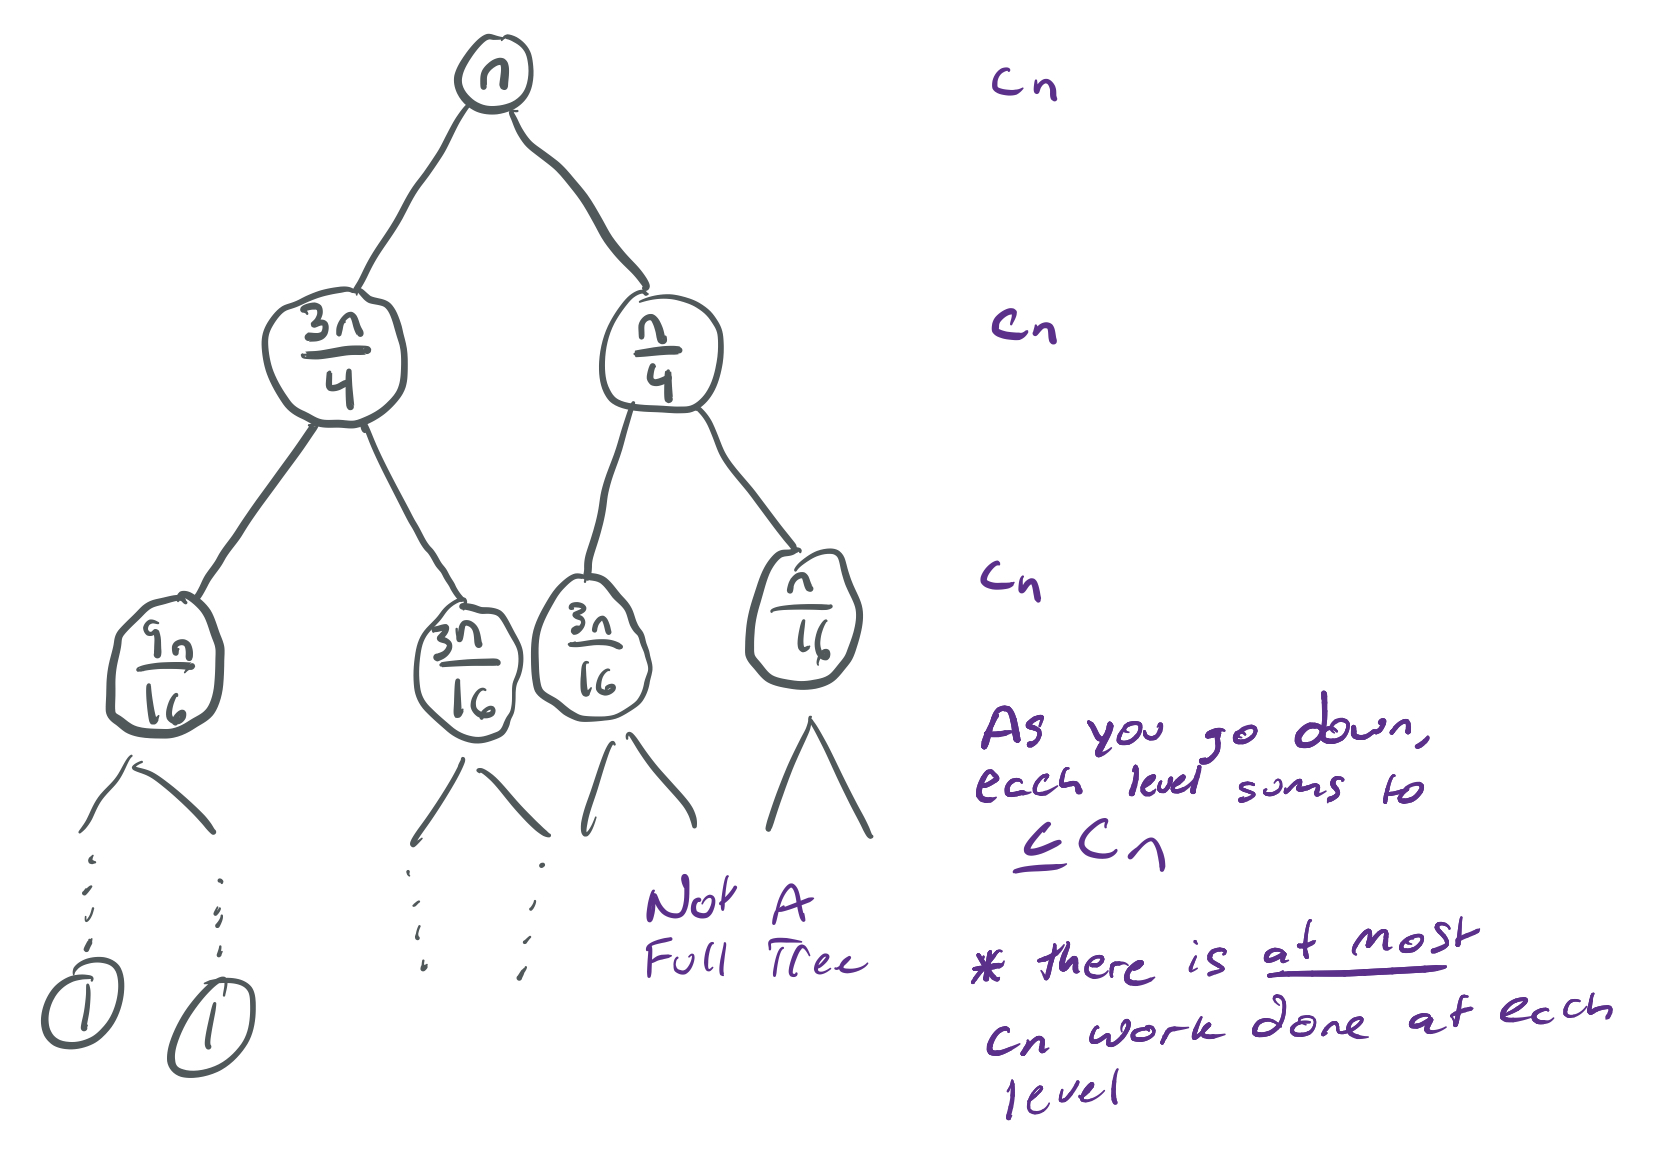
\includegraphics[scale=0.15]{hw5p1} 
		\end{center}
		$$\text{Recurrence Relation - } T(n) = T(\frac{3n}{4}) + T(\frac{n}{4}) + O(n)$$
		How many levels? - Longest path is when $ \left \lceil{\frac{n}{(\frac{4}{3})^k}}\right \rceil \leq 1 $ (k = number of levels)\\
		$$n \leq \left( 4/3 \right)^k$$
		$$ \log_{4/3}n \leq k$$
		$$ \log_{4/3}n + \epsilon = k  \text{ where } 0 \leq \epsilon < 1$$
		$$ \text{number of levels -}  \approx \log_{4/3}n $$
		$$ \text{Total work done}  \leq cn \log_{4/3}n$$
		$$ \text{Therefore } O(n \lg n)$$
		\item 
		K won't affect the big O time, but it will increase the average running time.		

\een
\fi
\newpage


%%%%%%%%%%%%%%%%%%%%%%%%%%%%%%%%%%%%%%%%%%%%%%%%%%%%%%%%
% PROBLEM TWO %% PROBLEM TWO %% PROBLEM TWO %% PROBLEM TWO %% PROBLEM TWO %
%==============================================================================
% Problem 2: Topic 2
%==============================================================================
% PROBLEM TWO %% PROBLEM TWO %% PROBLEM TWO %% PROBLEM TWO %% PROBLEM TWO %
%%%%%%%%%%%%%%%%%%%%%%%%%%%%%%%%%%%%%%%%%%%%%%%%%%%%%%%%
\vspace{5mm}
\item { \itshape 
	    (10 pts) Consider a chaining hash table $A$ with $b$ slots that holds data from a fixed, finite universe $U$. }
		\begin{enumerate}
		\item {\itshape (3 pts) State the simple uniform hashing assumption. }
		
		\item {\itshape (7 pts) Consider the worst case analysis of hash tables. Suppose we start with an empty hash table, $A$. A \textbf{collision} occurs when an element is hashed into a slot where there is another element already. Assume that $|U|$ represents the size of the universe and $b$ represents the number of slots in the hash table. Let us assume that $|U|\le b$. Suppose we intend to insert $n$ elements into $A$ \textbf{Do not assume the simple uniform hashing assumption for this subproblem.}
		\begin{enumerate}
	      \item What is the worst case for the number of collisions? Express your answer in terms of $n$.
	      \item What is the load factor for $A$ in the previous question?
	      \item How long will a successful search take, on average? Give a big-Theta bound.
	\end{enumerate}}
		
    \end{enumerate}
	\if\solutions1
\textbf{Solution:} \\
%==============================================================================
% STUDENTS: TYPE YOUR SOLUTIONS HERE. (Between \textbf{Solution:} and \fi )
%==============================================================================

\ben 
	\item 
		The simple uniform hashing assumption assumes that each of the slots in the hash table have an equal probability of being selected.
	\item
	\ben 
		\item \fbox{$n-1$} the first item will not collide, but every one after will collide.
		\item The load factor ($\alpha$) is defined to be $\frac{\text{number of items}}{\text{number of slots in table}}$, so in this case since we are talking about the worst case scenerio, there is only one slot in the table. Therefore, the load factor will be $\frac{n}{1} = \alpha = n$
		\item For hash tables with chaining, a successful search will take on average $\Theta (1+ \alpha)$ where $\alpha = \frac{\text{number of items}}{\text{number of slots in table}}$ So, the average successful search will be $\Theta \lp 1 + \frac{\text{number of items}}{\text{number of slots in table}} \rp$.\\
			This is proved in Prof. Cox's Lecture 9 - page 12, so I'm just working from that.
	\een 
\een


\fi
\newpage


%%%%%%%%%%%%%%%%%%%%%%%%%%%%%%%%%%%%%%%%%%%%%%%%%%%%%%%%
% PROBLEM THREE %% PROBLEM THREE %% PROBLEM THREE %% PROBLEM THREE %% PROBLEM THREE %
%==============================================================================
% Problem 3: Topic 3
%==============================================================================
% PROBLEM THREE %% PROBLEM THREE %% PROBLEM THREE %% PROBLEM THREE %% PROBLEM THREE %
%%%%%%%%%%%%%%%%%%%%%%%%%%%%%%%%%%%%%%%%%%%%%%%%%%%%%%%%

\vspace{5mm}

\item { \itshape 
	    (12 pts) Consider a hash table of size 100 with slots from 1 to 100. Consider the hash function $h(k) = \floor*{100k}$ for all keys $k$ for a table of size 100. You have three applications.
	    \begin{itemize}
	        \item \textbf{Application 1}: Keys are  generated uniformly at random from the interval $[0.3, 0.8]$.
	        \item \textbf{Application 2}: Keys are  generated uniformly at random from the interval $[0.1, 0.4] \cup [0.6, 0.9]$.
	        \item \textbf{Application 3}: Keys are  generated uniformly at random from the interval $[0, 1]$.
	    \end{itemize}
	}
		\begin{enumerate}
		\item {\itshape (3 pts) Suppose you have $n$ keys in total chosen for each application. What is the resulting load factor $\alpha$ for each application? }
		
		\item {\itshape (3 pts) Which application will yield the worst performance? }
		
		\item {\itshape (3 pts) Which application will yield the best performance? }
		
		\item {\itshape (3 pts) Which application will allow the uniform hashing property to apply? }
		
    \end{enumerate}
\if\solutions1
\vspace{2mm}




\if\solutions1
\vspace{2mm}




\if\solutions1
\vspace{2mm}

\textbf{Solution:} \\
%==============================================================================
% STUDENTS: TYPE YOUR SOLUTIONS HERE. (Between \textbf{Solution:} and \fi )
%==============================================================================
\ben 
	\item 
		\textbf{Application 1 - }\fbox{$\alpha = n/50$} \\ 
		\textbf{Application 2 - }\fbox{$\alpha = n/60$} \\
		\textbf{Application 2 - }\fbox{$\alpha = n/100$} \\	
	\item Application 1 will yield the worst performance since it has the smallest number of bins, leading to the largest load factor.
	\item Application 3 will yield the best performance since it has the largest number of bins, leading to the smallest load factor.
	\item Application 3 will allow the uniform hashing property to apply since it has 100 numbers, and 100 bins, all equally likely to be selected.
\een

\fi

\newpage

%%%%%%%%%%%%%%%%%%%%%%%%%%%%%%%%%%%%%%%%%%%%%%%%%%%%%%%%
% PROBLEM FOUR %% PROBLEM FOUR %% PROBLEM FOUR %% PROBLEM FOUR %% PROBLEM FOUR %
%==============================================================================
% Problem 4: Root and Ratio Test Review
%==============================================================================
% PROBLEM FOUR %% PROBLEM FOUR %% PROBLEM FOUR %% PROBLEM FOUR %% PROBLEM FOUR %
%%%%%%%%%%%%%%%%%%%%%%%%%%%%%%%%%%%%%%%%%%%%%%%%%%%%%%%%


\vspace{5mm}

\item{\itshape (12 pts) Median of Medians Algorithm
	}
	\begin{enumerate}%[label=(\alph)]
	
	\item{\itshape
    (4 pts) Illustrate how to apply the QuickSelect algorithm to find the $k = 4$th smallest element in the given array: \texttt{A = [5, 3, 4, 9, 2, 8, 1, 7, 6]} by showing the recursion call tree. Refer to  \href{https://canvas.colorado.edu/courses/69354/files/28668920?wrap=1}{Sam's Lecture 10} for notes on QuickSelect algorithm works }
    
    \item{\itshape
    (4 pt) Explain in 2-3 sentences the purpose of the Median of Medians algorithm.}
	
	\item{ \itshape
(4 pts)Consider applying Median of Medians algorithm (A Deterministic QuickSelect algorithm) to find the $4$th largest element in the following array: \texttt{A = [6, 10, 80, 18, 20, 82, 33, 35, 0, 31, 99, 22, 56, 3, 32, 73, 85, 29, 60, 68, 99, 23, 57, 72, 25]}.Illustrate how the algorithm would work for the first two recursive calls and indicate which sub array would the algorithm continue searching following the second recursion. Refer to \href{https://canvas.colorado.edu/courses/69354/files/28587193?wrap=1}{Rachel's Lecture 8} for notes on Median of Medians Algorithm}
		\end{enumerate}
\if\solutions1
\vspace{3mm}
{\bf Solution}: \\
%==============================================================================
% STUDENTS: TYPE YOUR SOLUTIONS HERE. (Between \textbf{Solution:} and \fi )
%==============================================================================

\ben
	\item \phantom{"nothing"}\begin{center}
		\textbf{NOTE - I'm using Sam's pseudocode, which would mean that for a k giving the 4th smallest element, k = 3. I'm 0 indexing it.}\\
		\phantom{"nothing"}\\
		Starting Array - \texttt{A = [5, 3, 4, 9, 2, 8, 1, 7, 6]}, \quad $k=3$\\
		Randomly Select a Pivot (using Siri to pick a random index 0-8) index = 1,\\ \textbf{pivot = A[1] = 3}\\
		Sort the array into two arrays, one of lower numbers, one of higher numbers -\\
		\texttt{Lower = [2, 1], Higher = [5, 4, 9, 8, 7, 6]}\\
		Since $k=3$, we enter the else of the if statement, therefore we recurse with the higher array, and $k = k-1 - $length(lower) $ = k = 0 $\\
		\phantom{"nothing"}\\\underline{Recurse}\\
		 Array - \texttt{A = [5, 4, 9, 8, 7, 6]}, \quad $k=0$\\
		 Randomly Select a Pivot (using Siri to pick a random index 0-5) index = 0,\\ \textbf{pivot = A[0] = 5}\\
		 Sort the array into two arrays, one of lower numbers, one of higher numbers -\\
		 \texttt{Lower = [4], Higher = [9, 8, 7, 6]}\\
		 Since $k=0$, we enter the first if statement, therefore we recurse with the lower array, and same $k=0$\\
		 \phantom{"nothing"}\\\underline{Recurse}\\
		 Array - \texttt{A = [4]}, \quad $k=0$\\
		 Since we have 1 item in the array, we return the item, returning 4\\
		 \phantom{"nothing"}\\
		 \fbox{4th Smallest Number = 4 according to QuickSelect}\\
		 \phantom{"nothing"}\\
		 Therefore the function returns $4$ which does confirm to be the 4th smallest element in the array once sorted by hand.
		 \phantom{"nothing"}\\\phantom{"nothing"}\\\phantom{"nothing"}\\\textit{B and C on next page}
		\end{center}
	
	\newpage
	\item
		The purpose of the Median of Medians algorithm is to select a better pivot than a random selection. By picking a pivot that is closer to the median of your data, you can divide the array into more even parts, causing there to be less recursions, making the algorithm faster. So by picking the median of medians, you may not be picking the actual median, but you will be picking something close, which can greatly decrease your running time.
	\item \phantom{"nothing"}\begin{center}
		\underline{Median of Medians -}\\
		Starting array - \\
	\texttt{A = [6, 10, 80, 18, 20, 82, 33, 35, 0, 31, 99, 22, 56, 3, 32, 73, 85, 29, 60, 68, 99, 23, 57, 72, 25]}
		\\\phantom{"nothing"}\\Divide array into sub arrays of size 5 (plus one array with remainders if any exist)
		\\\texttt{A = [6, 10, 80, 18, 20 | 82, 33, 35, 0, 31 | 99, 22, 56, 3, 32 | 73, 85, 29, 60, 68 | 99, 23, 57, 72, 25]}
		\\\phantom{"nothing"}\\Sort Each subarray (Sorting is $\Theta (n)$)
		\\\texttt{A = [6, 10, 18, 20, 80 | 0, 31, 33, 35, 82 | 3, 22, 32, 56, 99 | 29, 60, 68, 73, 85 | 23, 25, 57, 72, 99]}
		\\\phantom{"nothing"}\\Take the median of each subarray
		\\\texttt{A = [6, 10, \underline{18}, 20, 80 | 0, 31, \underline{33}, 35, 82 | 3, 22, \underline{32}, 56, 99 | 29, 60, \underline{68}, 73, 85 | 23, 25, \underline{57}, 72, 99]}
		\\Medians = \texttt{[18, 33, 32, 68, 57]}
		\\\phantom{"nothing"}\\Sort that subarray
		\\Medians = \texttt{[18, 32, 33, 57, 68]}
		\\\phantom{"nothing"}\\Take the median of medians
		\\Medians = \texttt{[18, 32, \underline{33}, 57, 68]}
		\\\phantom{"nothing"}\\\fbox{Median of Medians = 33}

		\phantom{"nothing"}\\\phantom{"nothing"}\\ \underline{Now use that value as a pivot in our quicksort algorithm}\\
		Starting array - \\
	\texttt{A = [6, 10, 80, 18, 20, 82, 33, 35, 0, 31, 99, 22, 56, 3, 32, 73, 85, 29, 60, 68, 99, 23, 57, 72, 25]}
		\\k = 4th largest element $ = k = 21$
		\\Pivot determined by Median of Medians = 33\\
		Sort the array into two arrays, one of lower numbers, one of higher numbers -\\
		\texttt{Lower = [6, 10, 18, 20, 0, 31, 22, 3, 32, 29, 23, 25], Higher = [80, 82, 35, 99, 56, 73, 85, 60, 68, 99, 57, 72]}\\
		Since $k=21$, we enter the else of the if statement, therefore we recurse with the higher array, and $k = k-1 - $length(lower) $ = k = 21 - 1 - 12 = 8$\\
		\phantom{"nothing"}\\\phantom{"nothing"}\\\textit{Continued on Next Page}
		
		\newpage\phantom{"nothing"}\\\textbf{Recurse}\\
		\phantom{"nothing"}\\
		\underline{Run Median of Medians on the new array - }\\
		Array - \texttt{A = [80, 82, 35, 99, 56, 73, 85, 60, 68, 99, 57, 72]}\\
		\phantom{"nothing"}\\Divide array into sub arrays of size 5 (plus one array with remainders if any exist)
		\\\texttt{A = [80, 82, 35, 99, 56 | 73, 85, 60, 68, 99 | 57, 72]}
		\\\phantom{"nothing"}\\Sort Each subarray (Sorting is $\Theta (n)$)
		\\\texttt{A = [35, 56, 80, 82, 99 | 60, 68, 73, 85, 99 | 57, 72]}
		\\\phantom{"nothing"}\\Take the median of each subarray
		\\\texttt{A = [35, 56, \underline{80}, 82, 99 | 60, 68, \underline{73}, 85, 99 | 57, \underline{72}]}
		\\Medians = \texttt{[80, 73, 72]}
		\\\phantom{"nothing"}\\Sort that subarray
		\\Medians = \texttt{[72, 73, 80]}
		\\\phantom{"nothing"}\\Take the median of medians
		\\Medians = \texttt{[72, \underline{73}, 80]}
		\\\phantom{"nothing"}\\\fbox{Median of Medians = 73}


		\phantom{"nothing"}\\\phantom{"nothing"}\\ \underline{Now use that value as a pivot in our quicksort algorithm}\\
		Starting array - \\
		Array - \texttt{A = [80, 82, 35, 99, 56, 73, 85, 60, 68, 99, 57, 72]}, \quad $k=8$\\
		Pivot determined by Median of Medians = 73\\
		Sort the array into two arrays, one of lower numbers, one of higher numbers -\\
		\texttt{Lower = [35, 56, 60, 68, 57, 72], Higher = [80, 82, 99, 85, 99]}\\
		Since $k=8$, we enter the else of the if statement, therefore we recurse with the higher array, and $k = k-1 - $length(lower) $ = k = 8 - 1 - 6 = 1$\\

		\phantom{"nothing"}\\\textbf{Recurse}\\
		\phantom{"nothing"}\\
		\underline{Run Median of Medians on the new array - }\\
		Array - \texttt{A = [80, 82, 99, 85, 99]}\\
		There's only 5 items, so sort array and find median\\
		\phantom{"nothing"}\\Sort Array -\\
		\texttt{A = [80, 82, 85, 99, 99]}\\
		\phantom{"nothing"}\\Find Median - \\
		\texttt{A = [80, 82, \underline{85}, 99, 99]}\\\phantom{"nothing"}\\
		\fbox{Since there is only one median, our median of medians is 85.}\\
		\phantom{"nothing"}\\\phantom{"nothing"}\\\textit{Continued on Next Page}
		\newpage
		\underline{Now use that value as a pivot in our quicksort algorithm}\\
		Starting array - \\
		Array - \texttt{A = [80, 82, 99, 85, 99]}\\
		Pivot determined by Median of Medians = 85\\
		Sort the array into two arrays, one of lower numbers, one of higher numbers -\\
		\texttt{Lower = [80, 82], Higher = [99, 99]]}\\
		\phantom{"nothing"}\\\phantom{"nothing"}\\Since $k = 1$ we enter the first if of the if statement, and would recurse with the lower array and same $k$ value.\\
		Example Call - \texttt{quickSelect([80, 82], 1)}

	\end{center}
		

	\een


\fi


%========================================================================================================================

\een 


\end{document}
